\chapter{Experiments}

    The purpose of this chapter is to overview the experiments phase of the project, which consists of the work done to deploy and measure how the system performs in a simulated scenario.
    Whereas the developed unit tests in the implementation stage aim to verify the correct functionality of separate units of code pertaining to the system, the execution of the entire system as a whole to serve a set of hypothetical use cases can help achieve a better grasp on how correct system functionality among all the tested units.
    Adjacent to the goal of testing the system in deployed scenarios, the experiments phase also aims to embed in the simulated environment a list of application scenarios that could leverage the ALTO system to its advantage, and subsequently observe and measure if and how the ALTO server can help the client in the form of provided resources that guide the client in taking application decisions that constitute a win-win scenario between the overlay and underlay.
    As comparison, other known application-network interaction strategies will also be observed and their results measured as a means to compare the impact that these strategies have on both layers.
    Findings on the state of the art of existing interactions and the proposal of the ALTO protocol made on section \ref{sec:state-of-art}, together with the specified system extension on \ref{sec:specification} leads one to believe that a theoretical mutually beneficial scenario exists in an ALTO approach that cannot exist with more asymmetrical means of interaction.
    This chapter, however, puts those theoretical scenarios into a practical environment that could be replicated by those reading this work, and exposing the created scenarios and collected data can corroborate the theoretical conclusions, as well as leaving an opportunity for future discussion on how the system behaved, including its performance, its success in aiding clients, other existing client options that could be a better route, system shortcomings, etc.
    This discussion benefits the ALTO project and can give more maturity to the system as it was put through a simulated deployment against other common strategies.

    The first section displays the chosen technologies for tasks pertaining to the experiments.
    The next section focuses on the required steps taken to setup the testing environment.
    This includes the design and deployment of a network topology in a simulated environment, the creation of mock applications to serve as clients for the system, and the design and deployment of application and network status measurement tools.
    The following section individually overviews the devised scenarios to test in the simulation, and with it experiment specifics such as the initial problem, what strategies will be tested to solve it, how many runs will be made per strategy, and what metrics will be measured.
    Finished the experiments, the following section will display the obtained results that were collected in the simulated environment, and the section after that will discuss these results and how they fare with the theoretical findings.

\section{Technologies Used}

    The Common Open Research Emulator (CORE) \cite{core} was used as a network simulator and represents the backbone of the experiments as a whole, as it represents the network simulator where the experimental environment will be set.
    This tool allows for the creation and emulation of network environments, and with it are included the abilities to construct network topologies and manipulate properties of the member nodes, which can include network routers, switches, and host machines, that will all be used for the designed experiment scenarios.
    Additionally, link connection properties can themselves be customized, as parameters like max bandwidth, packet loss percentage, or packet delay can be meticulously customized, and in fact will be in the upcoming scenarios as a means to simulate a given scenario that may occur in a realistic environment, such as link inefficiency resulting of peak traffic hours.
    Another property that was of great importance for its selection on this work is that, on top of the virtual network environment, arbitrary code can be run on behalf of a given entity and can be addressed to another, acting as if it were an actual network.
    This will be leveraged to run software pre-packaged in the emulator, such as routing protocols that are essential for the correct expected behavior of a simulator network, but also to schedule software execution that was developed for this work, which includes the ALTO server, network state providers - e.g., probing daemons and application feedback collectors - and system clients for the P2P and HTTP mock applications that will be devised to play out a particular experiment scenario, and which will have embedded into it an ALTO client to interface with the server for council.
    As the simulation tool runs on Linux and builds a simulated network that behaves very much like a real one, well known real-application tools can be used on top of it in other needed areas, including the deployment and measuring phases, which gives plenty of flexibility on tool selection.

    Python \cite{python} will be utilized to implement all simple software prototypes whose purpose is uniquely to test the application in a real scenario.
    This includes the P2P file-transfering applications, the HTTP servers and clients, and the throughput-intensive activities done by the data servers.
    Appended to this will also be the task of application monitoring, which includes the retrieval of performance statistics - doing so in the application's code itself, instead of using external tools, because more fine grained access exists and individual tasks can be monitored for how long and how well they perform.
    The choice of this programming language over others is simply that these software prototypes are not intended to be highly optimized, nor are they to be complex.
    Instead, their mode of operation is supposed to be simple in nature, to remove complex variables that might make the experiment results harder to interpret, and to make reasoning and replication of experiment results easier.
    Python seems then like a good fit due to its easy syntax, its interpreted nature that skips work that would otherwise be needed for compilation that might increase peformance - but is not needed - and, finally, its massive collection of helpful libraries.
    For these reasons will too Python be chosen to generate visual graphics reflective of the raw network and application statistics to be collected by other tools.

    Finally, a tool was selected for the task of network monitoring, to collect network data representative of the impact that a given application strategy had towards the infrastructure.
    To this goal, vnStat \cite{vnstat} was chosen, a command line utility to measure network traffic on an interface basis, over given periods of time.
    This application retrieves network interface statistics provided directly by the kernel, and thus performs no traffic sniffing.
    This is not problematic as this level of detail is not needed for the designed experiments, and instead interface statistics that inform on data flow influx and outflux are sufficient.
    Finally, with vnStat being a command line utility, there is the additional bonus that deployment and orchestration are facilitated with scripting.

    \textbf{[python's SimpleHTTPServer module will be leveraged as an HTTP server, and a similar module will be used for FTP file transfers.]}

\section{Setup}

    Figure \ref{fig:test-topology} displays the topology that will act as the main environment for all the devised experiments.
    It was designed with the intent of reflecting the nature of the Internet, in particular with it being an aggregation of multiple, heterogenous, domains, each with their own topological properties and internal policies, with them being administrated by different organizations.
    As can there be seen, a single backbone network - AS 0 - provides connectivity between many ASs and, to do its job correctly, a high degree of path redundancy exists between its edge routers, and the links have better capabilities that those associated with stub networks.
    AS 1 is a simple topological structure consisting of five PCs and and three dedicated servers, connected with the help of switches and routers, that eventually connect to a single edge router that connects to the backbone.
    AS 2 is representative of a data center with two OSPF areas, both constructed with a hierarchical organization common for data center networks.
    Links in these regions are also highly capable and high traffic peak times are expected to occur.
    AS 3 is a slightly more complex stub network compared to AS 1, but has the same structure, with the adition of having three OSPF areas instead of one, and a variety of nodes and links with different properties - for example, the links in area A are generally better, whilst area C has wireless connections in it that are expected to have worse performance and be less reliable.
    Finally, AS 4 connects directly with AS 3, meaning that the latter acts also as a transit AS, being the only access point towards the rest of the network.
    Similarly to AS 3, it consists of a stub network accessed by many end users and some servers, and both node and link properties vary accordingly.

    \todo{Add labels to autonomous systems and link and node properties}

    \begin{figure}[ht]
    \centering
    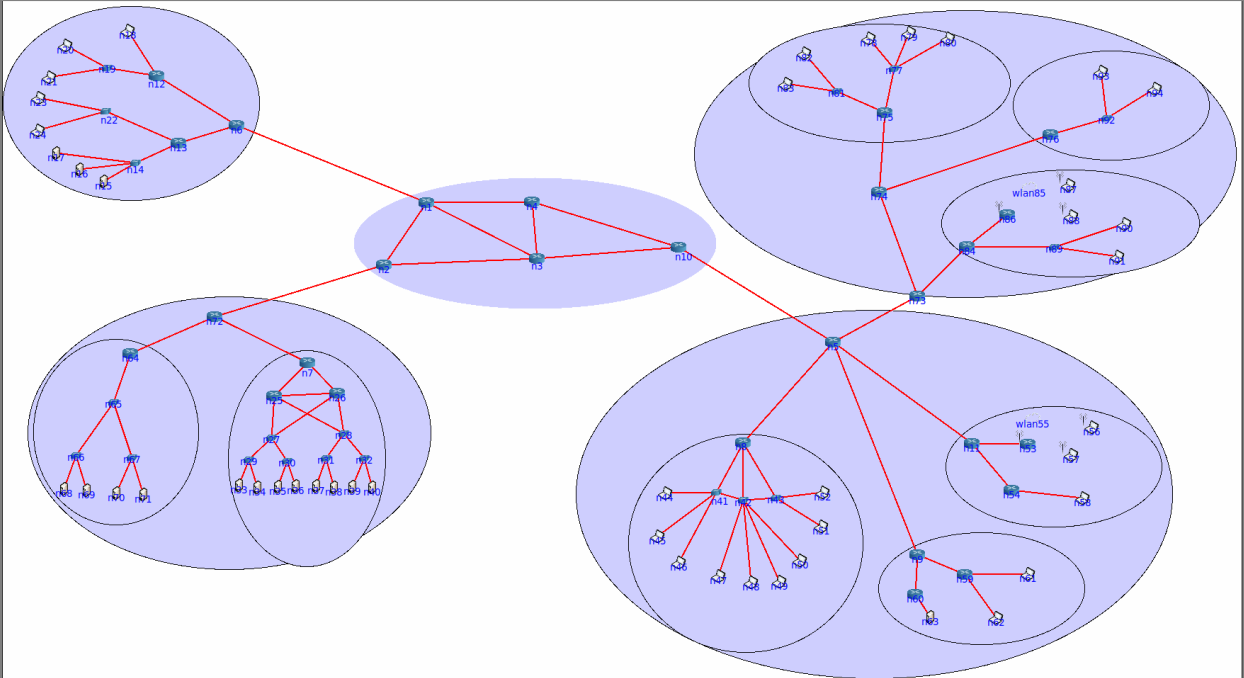
\includegraphics[scale=0.5]{img/test-topology.png}
    \label{fig:test-topology}
    \caption{Simulated topology environment}
    \end{figure}



    Each node on the network has a given purpose that is represented as a node label, and likewise are link labels used to specificy connection properties.
    Unless stated otherwise with these labels, all other properties are equal throughout the network.
    Some pre-packaged CORE services need to be enabled to assure network connectivity - mainly OSPFv3 and BGP - and scripting is used to, at the beginning of the simulation, bootstrap programs in specific nodes.
    This is done by leveraging the command line utility vcmd that runs specificed commands in control channels that are created at runtime by CORE - for example, the following command executes a ping command to address 10.0.0.1 with origins on node P2P-Cli-1 and on simulation session 12345:

    \begin{center}
    \begin{tabular}{c}
    \begin{lstlisting}[caption=Execution of an example command through the control channel of a given node, language=bash]
        $ vcmd -c /tmp/pycore.12345/P2P-Client-1 -- ping 10.0.0.1
    \end{lstlisting}
    \end{tabular}
    \end{center}

\section{Scenarios}

\subsection{Single ALTO administrative domain}

    The following experiments will consider a single ALTO server that only has administrative control of the AS it resides.
    It thus possesses no network topological details outside of his domain, working only with what it knows and what it can derive from the outside.

\subsubsection{Scenario 1 - P2P file sharing}
\textbf{Description:} All "Cli-N" nodes in the network, with N from 1 to N, actively serve all 10 equally sized fragments of a 1GB file to other peers, and the bootstrapping method includes informing the tracker about what file fragments they serve.
    "CliN-1" wishes to retrieve that file, and to do so he firstly contacts "Tracker" for tracking information about that file, that contains a mapping between a fragment ID and suggested peer, alongside with the file's checksum.
    After retreving this mapping, the client will sequencially request each fragment from the appointed peer, and afterwards merge all the fragments into a single file and validates that the calculated checksum matches the tracker's.
    An ALTO server is in the same AS and maintains a network map resource that groups endpoint addresses within locality - per OSPF area in the most specific pids, inside that AS in another, and anything else in another.


\textbf{Variables:} The variable actions to be tested are how the tracker selects a candidate peer to serve a fragment to the requesting peer.
Table \ref{table:s1-tracker-methods} displays the different tracker algorithms that will be tested for the task of peer matching.

\begin{table}[]
\begin{tabular}{ll}
Tracker Algorithm & Description                                                                                                                                                                                                \\
Random            & Randomly select among all available peers                                                                                                                                                                  \\
ALTO              & Retrieve a network map from its ALTO server and discover the attributed PID to both request and candidate clients, choosing randomly between the candidate peers that share the same PID as the candidate.
\end{tabular}
\label{table:s1-tracker-methods}
\end{table}

\textbf{Measurements:} Table \ref{table:s1-measurements} presents the measurements that will be collected during the experiment runs.

\begin{table}[]
\begin{tabular}{lll}
Measurement     & Units     & Description                                                  \\
Transfer Time   & Seconds   & Total amount of time required to transfer all file fragments \\
Network Traffic & Megabytes & Total amount of traffic that passed through the network
\end{tabular}
\label{table:s1-measurements}
\end{table}

\textbf{[Notes: The P2P client has no reasonable way to, without ISP cooperation, know that peers reside within network locality. A cited study used RTT heuristics that assumed that high RTT values exist in inter-ISP links, which may not always be the case. Randomly selecting is poor at optimal choice, but at the very least has potential for load balancing, something that the tracker itself can attempt to do on a per-locality basis, joining a best of both worlds. Leveraing only a network map to communicate peer locality is quick and takes little memory, and further experiments will add cost maps on top of it to mix both locality standards and QoS needs.]}


\subsubsection{HTTP file sharing}

\textbf{Description: } All "HTTP-N" nodes, with N from 1 to N, are HTTP servers and serve a 1GB file to querying clients.
Cli-N has a file that contains the address of all of these mirror servers on the network that can provide that given file to him.
The HTTP servers reside in the same AS, and that ALTO server maintains a network map that groups server regions of similar properties, an endpoint property map that provides real-time status information that includes current cpu and memory load, as well as a cost map providing throughput and delay costs that are compiled from voluntarily provided application performance statistics, as well as a routing cost specifying ISP preference.

\textbf{Variables: } The variable action to be tested is how the HTTP client selects between all known server mirrors that serve the desired file.
Table \ref{table:s2-clients-methods} displays the different client algorithms that will be tested for the task of server selection.

\begin{table}[]
\begin{tabular}{ll}
Client Algorithm & Description                                                                                                                                                                                                \\
Random            & Randomly select among all available servers                                                                                                                                                                  \\
Probe             & Probe for available TCP throughput and existing delay between all available servers, and select the one with most throughput with delay below 20 ms
                                                             \\
ALTO              & Retrieve a network map, endpoint property map, and cost map from the ALTO server in the HTTP servers AS, and choose, if possible, a server that is not overloaded - i.e., whose memory and cpu loads are not past 90\% - whose delay is below 20ms, and which has an historical throughtput of 30 Mbps or more.
If multiple servers match these requirements, choose the one that has the least routing cost among them.
\end{tabular}
\label{table:s1-tracker-methods}
\end{table}

\textbf{Measurements:} Table \ref{table:s2-measurements} presents the measurements that will be collected during the experiment runs.

\begin{table}[]
\begin{tabular}{lll}
Measurement         & Units      & Description                                                  \\
Transfer Time       & Seconds    & Total amount of time required to transfer the requested file \\
CPU Server Load     & Percentage & Average CPU load of all mirror servers \\
Memory Server Load  & Percentage & Average Memory load of all mirror servers \\
Network Traffic     & Megabytes  & Total amount of traffic that passed through the network
\end{tabular}
\label{table:s2-measurements}
\end{table}

\textbf{[Notes: The ALTO method has better data on three fronts: it has a historical and statistical record of connection quality between clients and servers, which will probably be more mature than a ad-hoc probing of the network at that given time; it has server property information regarding status (cpu and memory load, for example) that the client can't retrieve otherwise; it has ISP routing costs that give ISP insight on what choice would be more economically sound for them. The assumption is that the ALTO approach will have better application performance and better network resource utilization because the information retrieved tells a bigger picture than a simple probing for tcp througput and delay. Additionally, if every client were to perform adhoc measurements to pick a client, considerable network traffic overhead will exist, specially with a bigger scale of clients. By centralizing this information as historical and statistical data, and adding into it routing costs that only the ISP could derive, a more mature choice can exist that favors both parties. The old way of manually choosing server mirrors, for example for linux distributions, that end up just being 'let me choose the first one i see that is on my country', can be argued to be objectively worse than adding a ISP cooperative module.]}


\subsubsection{Bulk FTP transfers}

\textbf{Description:} Servers in the Data server AS want to schedule big data transfers between themselves as a form of backup.
These happen routinely, and take a predictable amount of time.
Performing these backups heavily impacts the ability of all servers in that data center to serve clients, because that subnetwork will be utilizing a lot of its resources to achieve that goal.
"Cli-N" wishes to retrieve a single 1GB file, and contains a file that lists all available mirrors and their address.
The data center administrator maintains a cost map calendar where he registers all scheduled backup transfers with two purposes: to keep track of all scheduled transfers so further ones cna be schedules as to not clash with pre-reserved ones, and to signal to ALTO clients when QoS levels to those servers are expected to degrade.

\textbf{Variables: } The variable action to be tested is how the HTTP client selects between all known server mirrors that serve the desired file.
Table \ref{table:s4-clients-methods} displays the different client algorithms that will be tested for the task of server selection.

\begin{table}[]
\begin{tabular}{ll}
Client Algorithm & Description                                                                                                                                                                                                \\
Random            & Randomly select among all available servers                                                                                                                                                                  \\
Probe             & Probe for available TCP throughput and existing delay between all available servers, and select the one with most throughput with delay below 20 ms
                                                             \\
ALTO              & Retrieve a network map and cost map from the ALTO server in the HTTP servers AS, and choose the one that maximizes throughput in the calendar entry where the transfer will occur.
\end{tabular}
\label{table:s5-tracker-methods}
\end{table}

\textbf{Measurements:} Table \ref{table:s1-measurements} presents the measurements that will be collected during the experiment runs.

\begin{table}[]
\begin{tabular}{lll}
Measurement     & Units     & Description                                                  \\
Transfer Time   & Seconds   & Total amount of time required to transfer all file fragments \\
Network Traffic & Megabytes & Total amount of traffic that passed through the network
\end{tabular}
\label{table:s1-measurements}
\end{table}

\subsection{Multi ALTO administrative domains}

    The following experiments assume that the ALTO synchronization protocol is in place and allows multiple servers to maintain globally scoped resources that can be shared to clients.

\subsubsection{P2P file transfer}

\textbf{Description:} Similar to the single domain counterpart, all "Cli-n" nodes in the network, with N from 1 to N, actively serve all 10 equally sized fragments of a 1GB file to other peers, informing the tracker of their availability to do so.
"CliN-1" wishes to retrieve that file, and to do so firstly contacts "Tracker" for tracking information about that file, that contains a mapping between fragment ID and suggested peer, alongside with the file's checksum.
    After retreving this mapping, the client will sequencially request each fragment from the appointed peer, and afterwards merge all the fragments into a single file and validates that the calculated checksum matches the tracker's.
    Each AS has an ALTO server operating with administrative control and topological insight of their own domain, and they together maintain a single cost map with global scope.

\textbf{Variables: } The variable actions to be tested are how the tracker selects a candidate peer to serve a fragment to the requesting peer.
Table \ref{table:s-tracker-methods} displays the different tracker algorithms that will be tested for the task of peer matching.

\begin{table}[]
\begin{tabular}{ll}
Tracker Algorithm & Description                                                                                                                                                                                                \\
Random            & Randomly select among all available peers                                                                                                                                                                  \\
ALTO              & Retrieve an endpoint cost map from its ALTO server that displays cumulative delay, available throughput, and routing cost between peers as a combined synchronization effort between ALTO domains.
Choose the candidate peer whose delay does is, if possible, below 20ms, with a throughput of 30 Mbps or more.
If multiple candidate peers fulfill these requirements, choose the one with the least amount of routing cost.
\end{tabular}
\label{table:s1-tracker-methods}
\end{table}

\textbf{Measurements:} Table \ref{table:s1-measurements} presents the measurements that will be collected during the experiment runs.

\begin{table}[]
\begin{tabular}{lll}
Measurement     & Units     & Description                                                  \\
Transfer Time   & Seconds   & Total amount of time required to transfer all file fragments \\
Network Traffic & Megabytes & Total amount of traffic that passed through the network
\end{tabular}
\label{table:s1-measurements}
\end{table}

\subsubsection{P2P media streaming}

\texbtf{Description: } All "Cli-N" nodes, with N from 1 to N, allow for real-time streaming of a given piece of media.
"Cli-N" has a file containing a list of all available peer addresses that he can request a feed to.

\textbf{Variables: } The variable actions to be tested are how the client selects a candidate peer to request a stream from.

\textbf{[Methods: a) ALTO server maintains a multi-domain throughput, delay and packet loss calendared cost maps that were result of historical and statistical measurements from previous users of that media streaming application that volunteered performance statistics. Routingcost calendared cost map is also added by the ISPs to reflect preference in routing. b) Randomly select peer. c) Choose peer with least RTT, with the heuristic that smallest probe delay allows for better real-time streaming experience d) Randomly select peer and, whenever QoS measurements are degraded for too long, choose another ano - and continuously apply this adaptive peer selective mechanism that essentially "brute forces" the best peer]}
\textbf{[Notes: Again, the ALTO approach is the only one that allows clients to make choices that are inline with ISP's economical and administrative needs. Moreso, the ALTO server has a centralized repository for historical and statistical performance results that occured in that media application, that show a trend in what subnetworks become more loaded over time. ISP probing by the network can also more quickly detect link bottlenecks and quickly upload that data as cost maps, whilst deducing that information without ISP aid would require more probing traffic, and would take considerably longer. Both probing attempts and "brute force" attempts are more harduous and considering the real-time QoS levels of the media streaming application, will considerably degrade application performance. A network-aware and statistical repository solution like ALTO allows one to make the better decision, more quickly, with a mutually beneficial outcome.]}

\section{Results}
\section{Discussion}

